\documentclass{standalone}
\usepackage{tikz}
\usepackage{ctex,siunitx}
\setCJKmainfont{Noto Serif CJK SC}
\usepackage{tkz-euclide}
\usepackage{amsmath}
\usetikzlibrary{patterns, calc}
\usetikzlibrary {decorations.pathmorphing, decorations.pathreplacing, decorations.shapes,}

\usetikzlibrary{decorations.pathmorphing,calc,shapes,shapes.geometric,patterns}
\tikzset{
  treetop/.style = {decoration={random steps, segment length=0.4mm}, decorate},
  trunk/.style   = {decoration={random steps, segment length=2mm,
                    amplitude=0.2mm}, decorate}}

\tikzset{
   my tree/.pic={
     \foreach \w/\f in {0.3/30,0.2/50,0.1/70} {
       \fill [brown!\f!black, trunk] (-\w/2,0) rectangle +(\w,3);
     }
     \foreach \n/\f in {1.4/40,1.2/50,1/60,0.8/70,0.6/80,0.4/90} {
       \fill [green!\f!black, treetop](0,3) ellipse (\n/1.5 and \n);
     }
   }
}

\begin{document}
\small
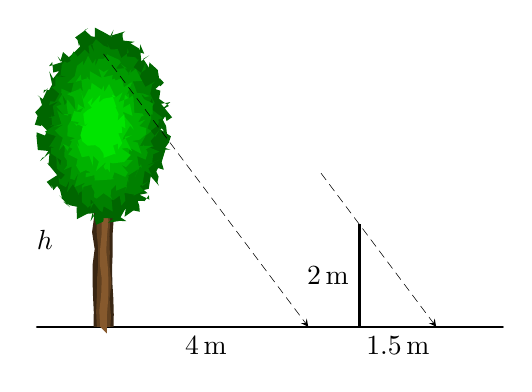
\begin{tikzpicture}[>=stealth,scale=0.65]
  \tkzSetUpPoint[fill=black]
  % \useasboundingbox(-1,-0.75)rectangle(3.7,1.4);
  \tkzDefPoints{0/0/A,4/0/B,5/0/C,6.5/0/D,0/5.33/E,5/2/F}
  \tkzDrawLine[thick](A,D)
  \pic at (0,0) [scale=0.85]   {my tree};
  \draw[very thick](C)--(F)node[midway,left]{\qty{2}{m}};
  \node at(5.75,0)[below]{\qty{1.5}{m}};
  \node at(2,0)[below]{\qty{4}{m}};
  \node at(-.8,1.7)[left]{$h$};
  \tkzDrawLine[densely dashed,add=0.5 and 0,->](F,D)
  \tkzDrawLine[densely dashed,add=0 and 0,->](E,B)
\end{tikzpicture}
\end{document}